%\documentclass[spanish]{beamer}

\documentclass{beamer}
\usepackage{pgf,pgfpages}
%\pgfpagesuselayout{4 on 1}[letterpaper,landscape,border shrink=0.5in]
\usepackage{algorithm,algorithmic}
%\usepackage{algorithm,algorithmicx}
%\usepackage[noend]{algpseudocode}
\usepackage{listings}
\lstset{basicstyle=\ttfamily,
	showstringspaces=false,
	commentstyle=\color{red},
	literate={á}{{\'a}}1
	{ã}{{\~a}}1
	{é}{{\'e}}1
	{É}{{\'E}}1
	{ó}{{\'o}}1
	{í}{{\'i}}1
	{ñ}{{\~n}}1
	{¡}{{!`}}1
	{¿}{{?`}}1
	{ú}{{\'u}}1
	{Í}{{\'I}}1
	{Ó}{{\'O}}1
}

\usepackage{beamerthemesplit}
\usepackage{color}
\usepackage[utf8]{inputenc}
\usepackage[spanish]{babel}
%\usepackage[latin1]{inputenc}
%\usepackage[pdftex]{graphicx}
%\usepackage{algorithm}
%\usepackage{algorithmic-C}
%\usepackage{algorithmic}
\usepackage{amsthm}
\usepackage{multicol}
\usepackage{multirow}
\usepackage{fancyvrb,relsize}
\usepackage{hhline}
\usepackage{tikz}
\usetikzlibrary{trees, shapes, calc}
\newcommand{\inputTikZ}[2]{%
	\scalebox{#1}{\input{#2}}
}

\usetheme{Warsaw} %Gueno
%\usetheme{Darmstadt} %OK!
% \usetheme{Frankfurt} %OK!
%\usetheme{Goettingen}
%\usetheme{Dresden}
%\usetheme{JuanLesPins} %OK!!
%\usetheme{Marburg}
%\usetheme{Montpellier}
%\usetheme{Rochester} %sobrio
%\usetheme{Singapore}
%\usetheme{Szeged}

%\usecolortheme{albatross}
%\usecolortheme{seahorse}
%\usecolortheme{beetle}
%\usecolortheme{crane}
%\usecolortheme{dolphin}
%\usecolortheme{dove}
%\usecolortheme{fly}
%\usecolortheme{lily} %Gueno
\usecolortheme{orchid}%Gueno
%\usecolortheme{rose}
%\usecolortheme{seagull}
%\usecolortheme{whale}


\DefineVerbatimEnvironment%
      {VerbatimNN}%
      {Verbatim}%
      {fontsize=\relsize{-1}}
\DefineVerbatimEnvironment%
      {VerbatimNNN}%
      {Verbatim}%
      {fontsize=\relsize{-2}}

\DefineVerbatimEnvironment%
      {VerbatimPseudo}%
      {Verbatim}%
      {numbers=left, fontsize=\relsize{-1}}
\DefineVerbatimEnvironment%
      {VerbatimPseudoReduced}%
      {Verbatim}%
      {numbers=left, fontsize=\relsize{-2}}
\DefineVerbatimEnvironment%
      {VerbatimPseudoReduced2}%
      {Verbatim}%
      {numbers=left, fontsize=\relsize{-3}}
\DefineVerbatimEnvironment%
      {VerbatimC}%
      {Verbatim}%
      {commandchars=@ªº, numbers=left, fontsize=\relsize{-1}}
\DefineVerbatimEnvironment%
      {VerbatimReducedC}%
      {Verbatim}%
      {commandchars=@ªº, numbers=left, fontsize=\relsize{-2}}
\DefineVerbatimEnvironment%
      {VerbatimReduced2C}%
      {Verbatim}%
      {commandchars=@ªº, numbers=left, fontsize=\relsize{-3}}



%\AtBeginSubsection[]
%{
% \begin{frame}
% \frametitle{Sinopsis}
% Aqui decides: cada seccion y subseccion:
% \tableofcontents[currentsection,currentsubsection]
 %O solamente la seccion (Solo uno de ellos)
%\tableofcontents[currentsection]
% \end{frame}
%}

% Si quieres que todo por default aparezca de poco en poco
% descomenta esta linea
%\beamerdefaultoverlayspecification{<+->}

\setbeamertemplate{footline}{\hfill\insertframenumber/\inserttotalframenumber}
\setbeamertemplate{navigation symbols}{}

\setbeamercovered{transparent}

\title{ELO320 - Estructuras de Datos y Algoritmos\\Tipos de Datos Abstracts\\Pilas, Listas Circulares y Colas}
%\subtitle{Ingeniería Civil Telemática UTFSM}
\author{Dr. Nicolás Gálvez R.\\{\small nicolas.galvez@usm.cl}}
\institute{Ing. Civil Telemática - Departamento de Electrónica}
\titlegraphic{
\includegraphics[scale=.18]{images/logoutfsm}}
\date{2do Semestre 2022}

\begin{document}

\frame{\titlepage}

%\section*{Sinopsis}
%\frame{  \frametitle{Sinopsis}\tableofcontents[pausesections]}
%
%

\section{Recordando: Lista Simple Enlazada}

\begin{frame}[fragile]
 \frametitle{Lista Simple Enlazada: Inicializar}

Las listas, en su versión más básica, dependen de un puntero al inicio de la lista. Éste suele llamarse \textit{header}, \textit{cabecera} o  \textit{inicio}.
\begin{exampleblock}{C}
\begin{lstlisting}[language=C, basicstyle=\tiny, escapeinside={|}{|}]
#include<stdio.h>

typedef struct nodo{
	int dato; //dato, puede ser lo que uds. necesiten
	struct nodo *sgte; // puntero a un nodo enalce.
} nodo_t;

int main(int argc, char **argv){

	nodo_t * inicio = NULL; 
	// Inicializamos la lista, con su puntero de inicio apuntando a NULL
	// Equivalente a lista vacía []

	return 0;
}
\end{lstlisting}
\end{exampleblock}
\end{frame}

\begin{frame}[fragile]
 \frametitle{Lista Simple Enlazada: Inicializar}
\begin{center}
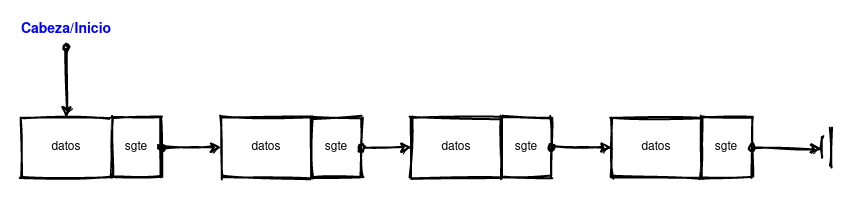
\includegraphics[width=.9\linewidth]{images/linkedlist1}
\end{center}

\end{frame}

\begin{frame}[fragile]
\frametitle{Lista Enlazada PRO}
Existen otras implementaciones de listas enlazadas simples, donde se incluyen más punteros y variables de control.

\begin{exampleblock}{C}
\begin{lstlisting}[language=C, basicstyle=\tiny, escapeinside={|}{|}]
#include<stdio.h>

typedef struct nodo{
	int dato; //dato, puede ser lo que uds. necesiten
	struct nodo *sgte; // puntero a un nodo enalce.
} nodo_t;

int main(int argc, char **argv){

	nodo_t * inicio = NULL; //pueden usar un struct para estos datos
	nodo_t * final = NULL;
	int largo = 0;
	// Equivalente a lista vacía []
	// ¿Para que sirve esta nueva forma?
	// Implemente las funciones de ésta clase considerando esta forma.

	return 0;
}
\end{lstlisting}
\end{exampleblock}
\end{frame}

\begin{frame}[fragile]
\frametitle{Lista Enlazada PRO}
\begin{center}
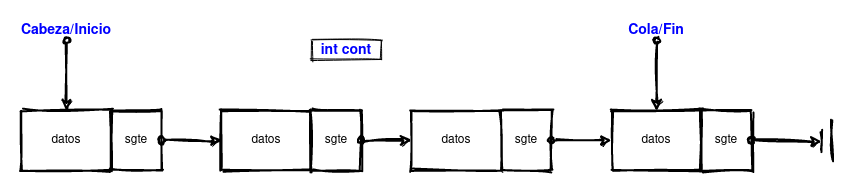
\includegraphics[width=.9\linewidth]{images/linkedlist2}
\end{center}
\end{frame}

\begin{frame}[fragile]
 \frametitle{Lista Doblemente Enlazada}

\begin{exampleblock}{C}
\begin{lstlisting}[language=C, basicstyle=\tiny, escapeinside={|}{|}]
#include<stdio.h>

typedef struct nodo{
	int dato; //dato, puede ser lo que uds. necesiten
	struct nodo *sgte; // puntero a un nodo siguiente, enalce.
	struct nodo *prev; // puntero a un nodo previo, enalce.
} nodo_t;

int main(int argc, char **argv){

	nodo_t * inicio = NULL; 
	// Inicializamos la lista, con su puntero de inicio apuntando a NULL
	// Equivalente a lista vacía []

	return 0;
}
\end{lstlisting}
\end{exampleblock}

\begin{center}
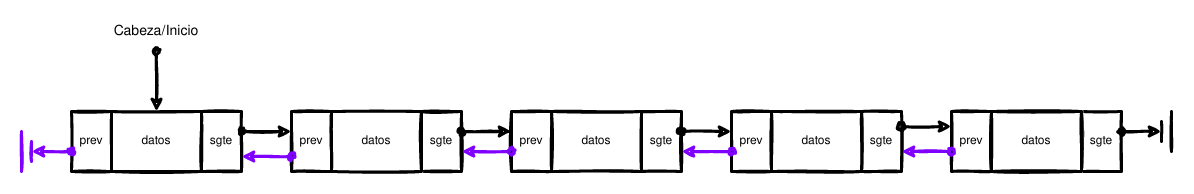
\includegraphics[width=0.95\linewidth]{images/doublelinkedlist1}
\end{center}
\end{frame}

\begin{frame}[fragile]
\frametitle{Lista Doblemente Enlazada PRO}
Existen otras implementaciones de listas enlazadas simples, donde se incluyen más punteros y variables de control.

\begin{exampleblock}{C}
\begin{lstlisting}[language=C, basicstyle=\tiny, escapeinside={|}{|}]
#include<stdio.h>

typedef struct nodo{
	int dato; //dato, puede ser lo que uds. necesiten
	struct nodo *sgte; // puntero a un nodo enalce.
} nodo_t;

int main(int argc, char **argv){

	nodo_t * inicio = NULL; //pueden usar un struct para estos datos
	nodo_t * final = NULL;
	int largo = 0;
	// Equivalente a lista vacía []
	// ¿Para que sirve esta nueva forma?
	// Implemente las funciones de ésta clase considerando esta forma.

	return 0;
}
\end{lstlisting}
\end{exampleblock}
\end{frame}

\begin{frame}[fragile]
\frametitle{Lista Doblemente Enlazada PRO}
\begin{center}
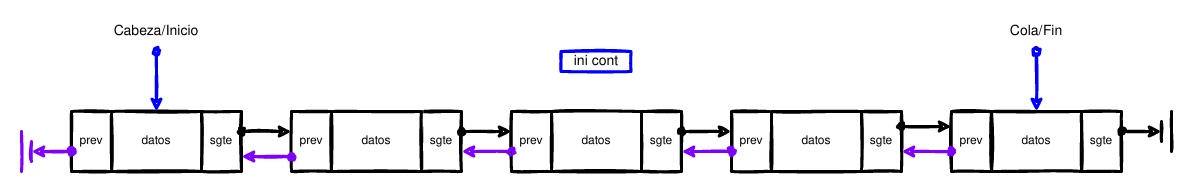
\includegraphics[width=\linewidth]{images/doublelinkedlist2}
\end{center}
\end{frame}

\begin{frame}[fragile]
\frametitle{Lista Doblemente Enlazada PRO+}
Existen otras implementaciones de listas enlazadas simples, donde se incluyen más punteros y variables de control.

\begin{exampleblock}{C}
\begin{lstlisting}[language=C, basicstyle=\tiny, escapeinside={|}{|}]
#include<stdio.h>

typedef struct nodo{
	int dato; //dato, puede ser lo que uds. necesiten
	struct nodo *sgte; // puntero a un nodo enalce.
} nodo_t;

int main(int argc, char **argv){

	nodo_t * inicio = NULL; //pueden usar un struct para estos datos
	nodo_t * final = NULL;
	nodo_t * actual = NULL;
	int largo = 0;
	int pos_actual = 0;
	// Equivalente a lista vacía []
	// ¿Para que sirve esta nueva forma?
	// Implemente las funciones de ésta clase considerando esta forma.

	return 0;
}
\end{lstlisting}
\end{exampleblock}
\end{frame}

\begin{frame}[fragile]
\frametitle{Lista Doblemente Enlazada PRO+}
\begin{center}
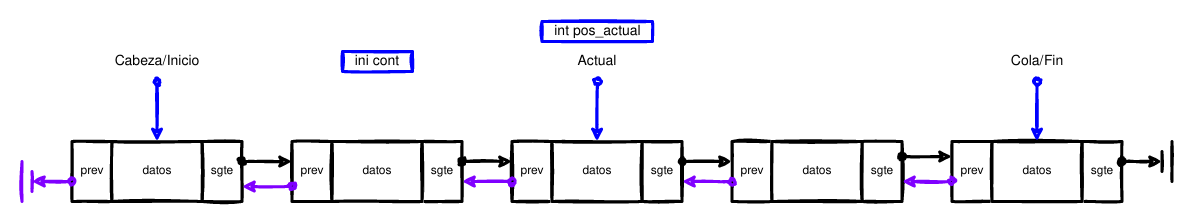
\includegraphics[width=\linewidth]{images/doublelinkedlist3}
\end{center}
\end{frame}

\section{Pilas o Stacks}
\begin{frame}[fragile]
\frametitle{Pilas o Stacks}
\small
La pila o stack es estructura de datos que permite operar solo en uno de sus extremos. Es de tipo \textbf{LIFO: Last In, First Out}. Puede ser implementada con arreglos o listas. 

\begin{center}
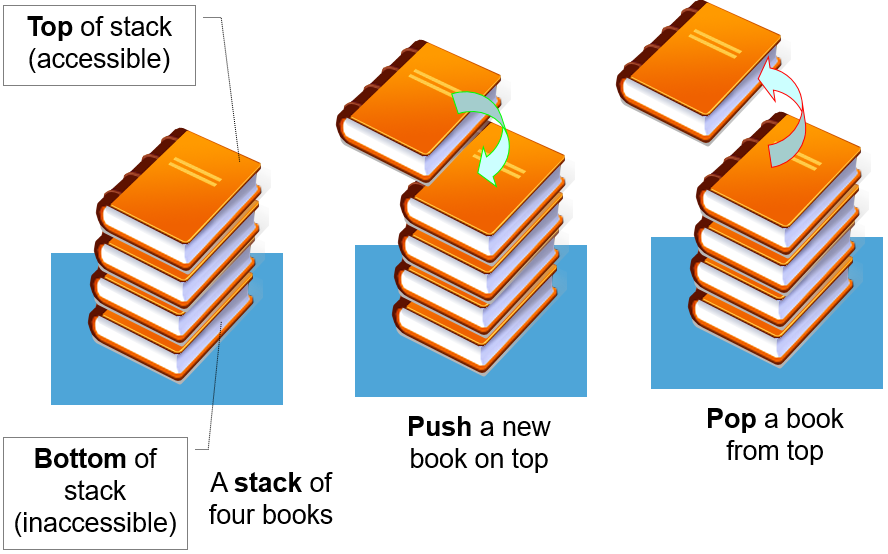
\includegraphics[width=0.5\linewidth]{images/stack_illustration}
\end{center}

Aplicaciones:
\begin{itemize}
\item Control+Z o Control+Y/Control+Mayus+Z: Operaciones de Desahcer o Rehacer (undo/redo).
\item Compilación: Formulas matemáticas en notacion de primer orden, i.e. $(x\ 1\ (+\ 2\ 3)) = x\ 1\ +\ 2\ 3$
\item Busqueda en árboles: Por ejemplo Búsqueda en Profundidad (Deep-first Search o DFS).
\end{itemize}
\end{frame}

\begin{frame}[fragile]
 \frametitle{Pilas o Stacks: Interfaz}
\begin{center}
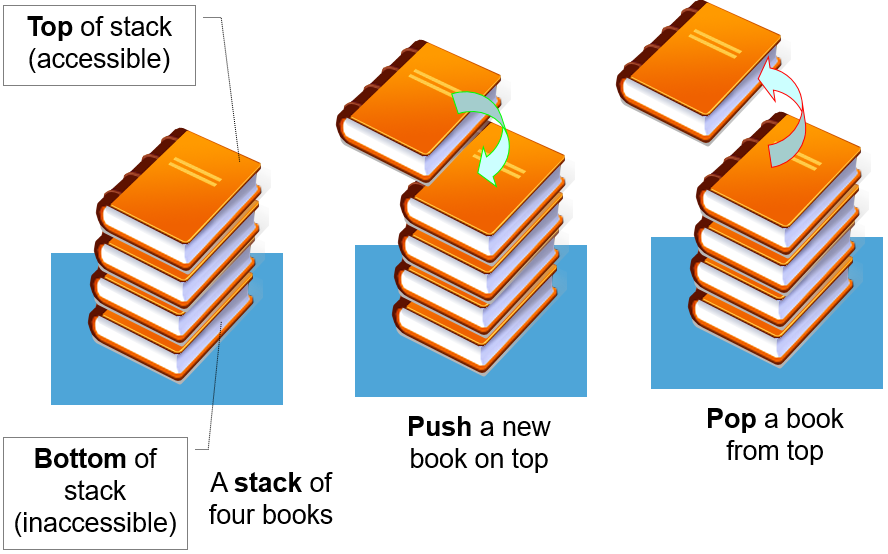
\includegraphics[width=0.5\linewidth]{images/stack_illustration}
\end{center}

\begin{itemize}
\item \texttt{push()}: Ingresa un nuevo elemento en la pila.
\item \texttt{pop()}: Elimina el elemento superior de la pila.
\item \texttt{peak()}: Devuelve el valor del primer elemento en la pila.
\item \texttt{is\_empty()}: Revisa si la pila está vacía.
\item \texttt{is\_full()}: Revisa si la pila está llena (solo para tamños fijos).
\item ¿Cómo se implementan? 
\end{itemize}
\end{frame}

\begin{frame}[fragile]
 \frametitle{Pilas o Stacks}
\begin{center}
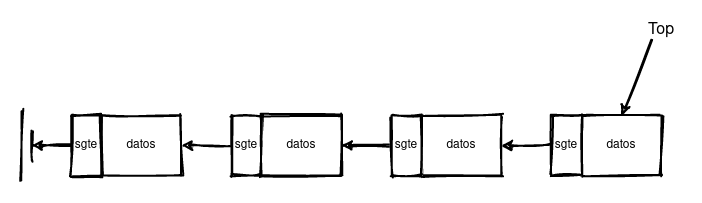
\includegraphics[width=0.95\linewidth]{images/stack-base}
\end{center}
\end{frame}


\begin{frame}[fragile]
 \frametitle{Pilas o Stacks: \texttt{push()}}
\begin{center}
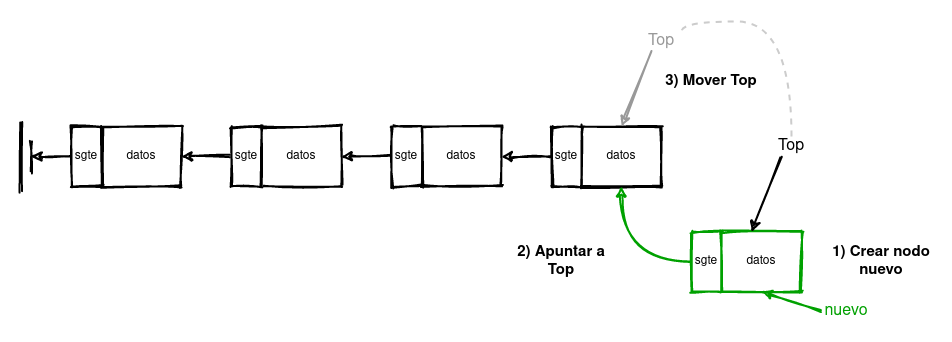
\includegraphics[width=0.95\linewidth]{images/stack-push}
\end{center}
\end{frame}

\begin{frame}[fragile]
 \frametitle{Pilas o Stacks: \texttt{pop()}}
\begin{center}
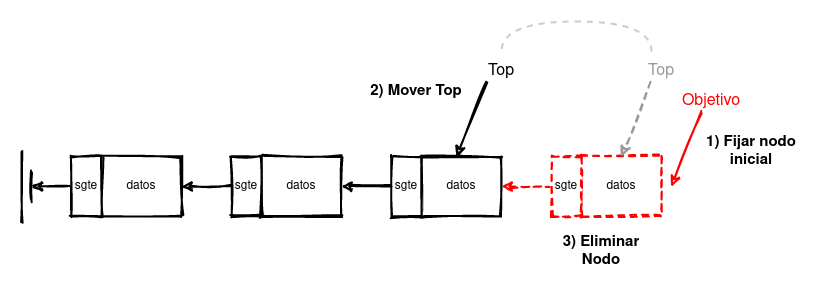
\includegraphics[width=0.95\linewidth]{images/stack-pop}
\end{center}
\end{frame}

\section{Listas Circulares}
\begin{frame}[fragile]
\frametitle{Listas Circulares}
La lista circular es una variación de la lista simple/doble enlazada en la cual, el primer elemento
está conectado con el último elemento, creando así una estructura circular.

\begin{center}
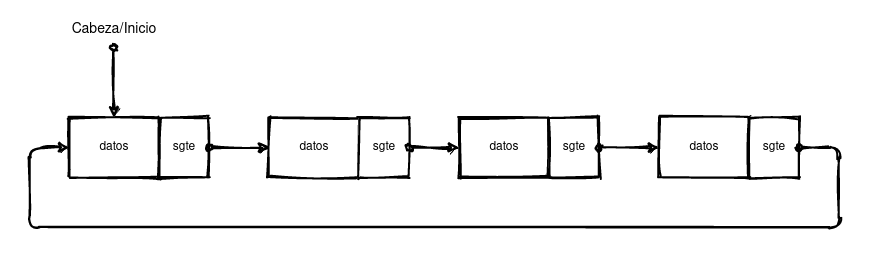
\includegraphics[width=0.75\linewidth]{images/circular-ll}
\end{center}
\begin{center}
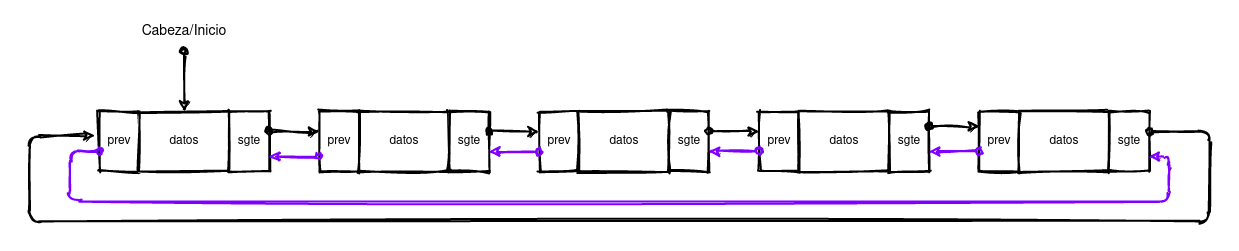
\includegraphics[width=0.95\linewidth]{images/circular-dll}
\end{center}
\end{frame}

\begin{frame}[fragile]
\frametitle{Listas Circulares}
Ventajas:
\begin{itemize}
\item Cualquier nodo puede ser la cabezera o final.  
\item Si una estructura tiene dos punteros, ahora solo es necesario uno.
\item Útil para lecturas reiterativas de elementos. 
\end{itemize}

Aplicaciones:
\begin{itemize}
\item Colas o Queues.
\item Buffers circulares dinámicos y estáticos.
\item Planificacion de ejecución de componentes de CPU.
\item Todo tipo de round robin scheduling.
\end{itemize}
\end{frame}

\section{Colas o Queues.}
\begin{frame}[fragile]
\frametitle{Colas o Queues}
\small
La cola o queue es una estructura de datos que permite operar en un extremo para entrada y en otro extremo para salida. Simula el comportamiento de una fila o cola. Es de tipo \textbf{FIFO: First In, First Out}. Puede ser implementada con arreglos o listas. 

\begin{center}
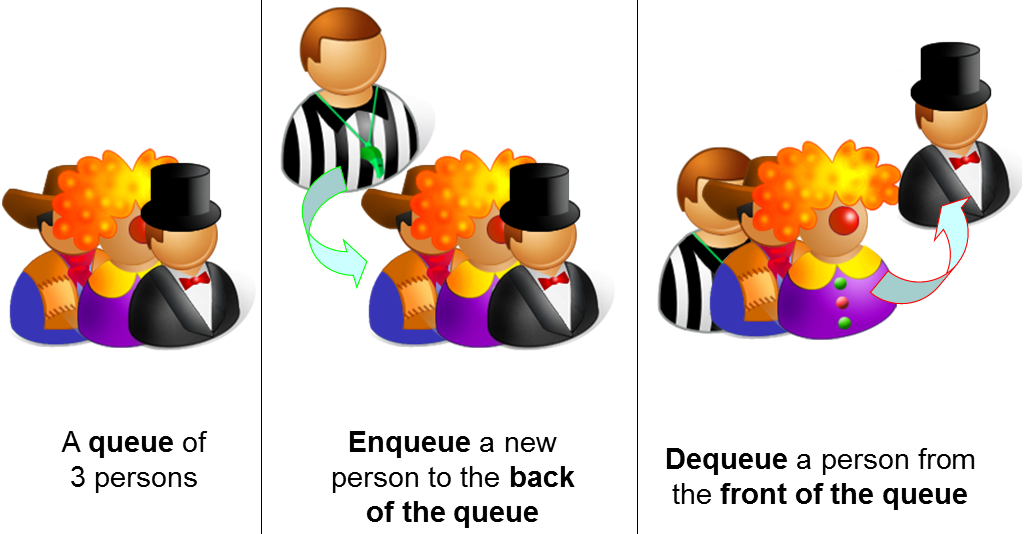
\includegraphics[width=0.5\linewidth]{images/queue_illustration}
\end{center}

Aplicaciones:
\begin{itemize}
\item Planificación de recursos. Priorización. 
\item Colas de impresión. 
\item Comunicación asincrónica e interrupciones de sistema.
\item Teoría de Colas. 
\end{itemize}

\end{frame}

\begin{frame}[fragile]
 \frametitle{Pilas o Stacks: Interfaz}
\begin{center}
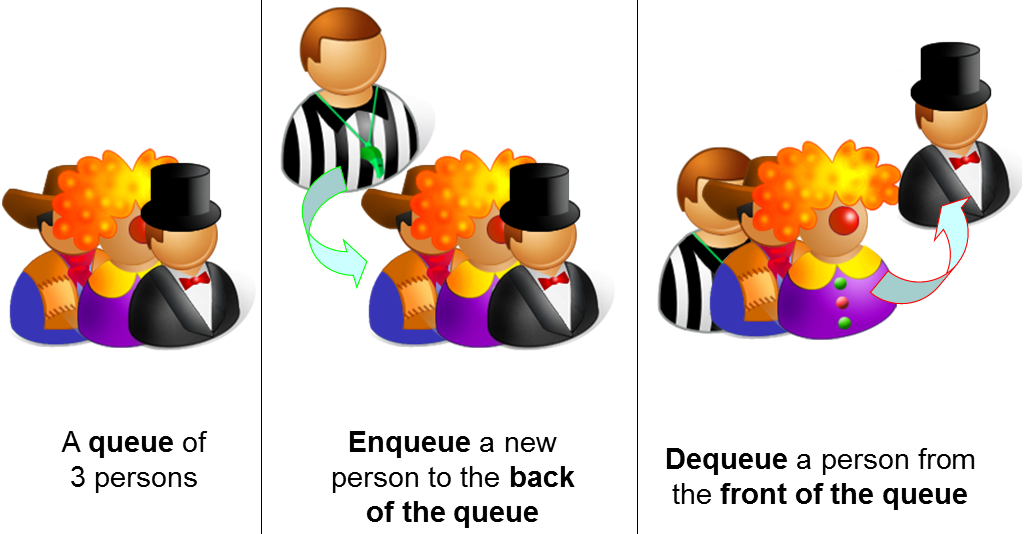
\includegraphics[width=0.5\linewidth]{images/queue_illustration}
\end{center}

\begin{itemize}
\item \texttt{enqueue()}: Ingresa un nuevo elemento al final de la cola.
\item \texttt{dequeue()}: Elimina el primer elemento de la cola.
\item \texttt{size()}: Devuelve el tamaño de la queue. 
\item \texttt{check()}: Devuelve el valor de un elemento de la cola.
\item \texttt{is\_empty()}: Revisa si la queue está vacía.
\item \texttt{is\_full()}: Revisa si la queue está llena (solo para tamños fijos).
\item ¿Cómo se implementan? 
\end{itemize}
\end{frame}

\begin{frame}[fragile]
\frametitle{Colas o Queues}
\begin{center}
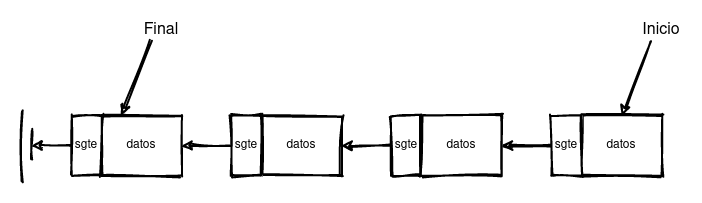
\includegraphics[width=0.95\linewidth]{images/queue1}
\end{center}
\end{frame}


\begin{frame}[fragile]
 \frametitle{Colas o Queues: \texttt{enqueue()}}
\begin{center}
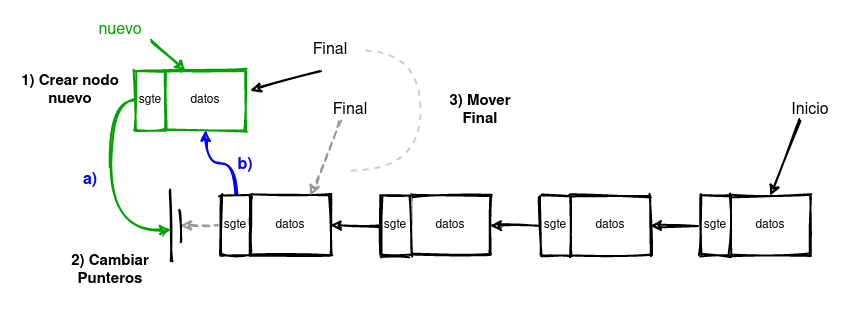
\includegraphics[width=0.95\linewidth]{images/enqueue1}
\end{center}
\end{frame}

\begin{frame}[fragile]
 \frametitle{Colas o Queues: \texttt{dequeue()}}
\begin{center}
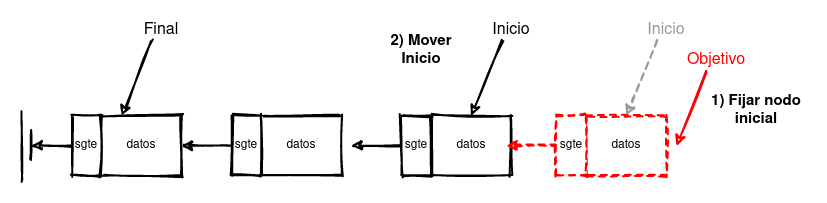
\includegraphics[width=0.95\linewidth]{images/dequeue1}
\end{center}
\end{frame}



\begin{frame}[fragile]
 \frametitle{Colas o Queues Circulares}
Es una fila o cola que se implementa utilizando estructuras de datos circulares, i.e., listas enlazadas circulares.\\

Ventaja principal, necesita sólo puntero para ser manejada, en la posición final. No hay necesidad de recorrer toda la fila para poder hacer cambios. 
\begin{center}
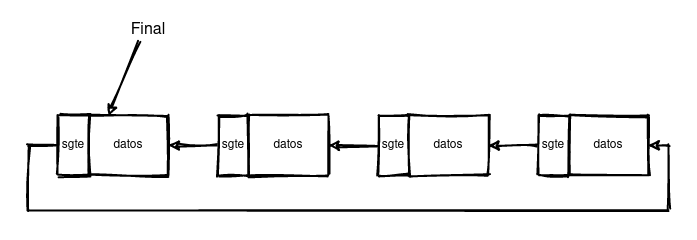
\includegraphics[width=0.95\linewidth]{images/queue2}
\end{center}
\end{frame}


\begin{frame}[fragile]
 \frametitle{Colas o Queues: \texttt{enqueue()}}
\begin{center}
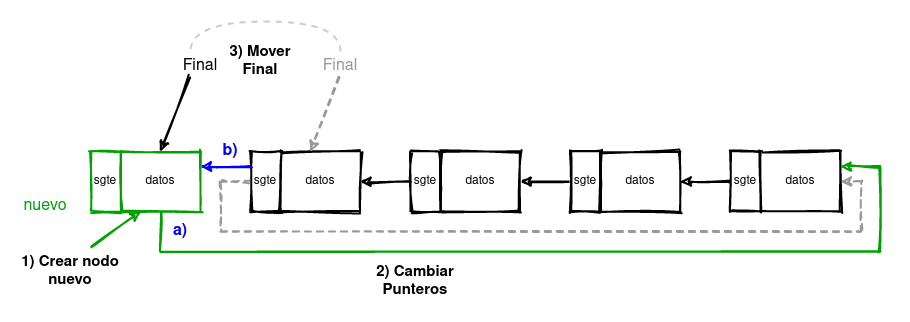
\includegraphics[width=0.95\linewidth]{images/enqueue2}
\end{center}
\end{frame}

\begin{frame}[fragile]
\frametitle{Colas o Queues: \texttt{dequeue()}}
\begin{center}
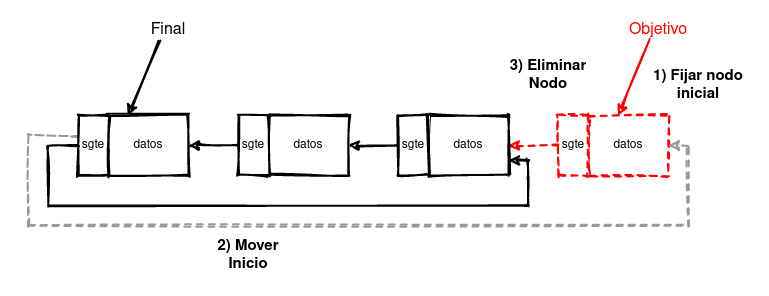
\includegraphics[width=0.95\linewidth]{images/dequeue2}
\end{center}
\end{frame}

\begin{frame}[fragile]
 \frametitle{Desafío}
Desarrolle un programa que:
\begin{itemize}
\item Invierta una palabra utilizando pilas.
\item Inveirta una palabra usando queues. 
\item Invierta una lista utilizando stacks.
\item Invierta una lista utilizando colas. 
\end{itemize}
\end{frame}


\end{document}
